\subsection{Perancangan Arsitektur Aplikasi}
	
      \begin{figure}[H]
        \centering
        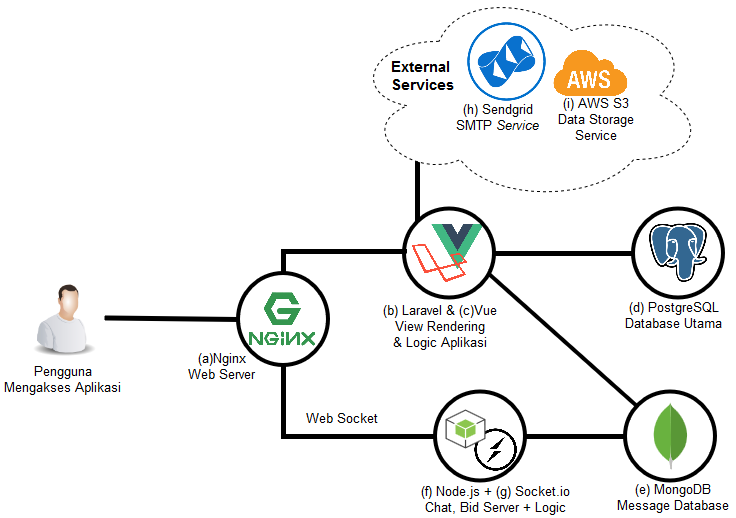
\includegraphics[width=\textwidth]{images/bab3/diagram/arsitektur-awal.png}
        \caption{Arsitektur Aplikasi Lelang \textit{online} 
        		\\
                \textit{External Services} artinya adalah menggunakan \textit{service} dari luar, tidak dibangun sendiri. }
        \label{arsitektur-app-final}
      \end{figure}
    
    \subsubsection{\textbf{\textsc{Nginx} sebagai WebServer dan Proxy Server}}
    {\scshape Nginx} adalah \textit{web} server multifungsi - dimana selain berfungsi sebagai Webserver, namun juga bisa berfungsi sebagai Load Balancer. Dalam awal pembuatan aplikasi, \textsc{Nginx} hanya digunakan sebagai \textit{web server} untuk melayani permintaan halaman \textit{web} dari pengguna.
    \\
    Namun, saat \textit{deployment}, banyak sekali terjadi \textit{issue} yang berkaitan dengan \textit{ssl certificate}, sehingga pada akhirnya Nginx juga digunakan sebagai \textit{proxy server} - dimana Nginx mempunyai fungsi baru yaitu \textit{redirecting request=request} yang masuk ke dalam server, dan meneruskannya ke proses dalam server yang bertugas memproses \textit{request} tersebut.
	   \\
    Beberapa masalah yang ditemukan penulis, jika tidak menggunakan fitur \textsc{Nginx} sebagai proxy server untuk aplikasi Soket yang berbeda port adalah sebagai berikut :
	    \begin{itemize}[noitemsep,topsep=0pt]
	    \item CORS (Cross Origin Reference Source)
	    \newline
	    Dimana pada saat browser mengakses soket dari port lain (meskipun domainnnya sama), browser menganggap bahwa sambungan dari port lain tersebut sebagai \textit{security threat} dan otomatis memutuskan sambungan.
	    \item ERROR :: INSECURE RESPONSE!
	    \newline
	    Hal ini terjadi saat browser membuka sebuah \textit{web} dengan https - namun mengakses koneksi soket yang tidak terproteksi dengan https. Hal ini juga membuat browser menganggap ini sebagai \textit{security threat}, dan tidak membuka \textit{reply} dari koneksi soket yang tidak terproteksi dengan https tersebut.
	    \end{itemize}
    
    \subsubsection {\textbf{Laravel dan Logika Aplikasi}}
    \textsc{Laravel}, bertugas sebagai Bos Besar, pengelola data dan manajemen data, dan pelayan \textit{request} dalam aplikasi Lelang \textit{online} ini. Semua request diteruskan, dan diproses oleh \textsc{Laravel}, dan diproses oleh Laravel. 	    
    
    \subsubsection{\textbf{Vue.js sebagai \textit{View Renderer} }}
	Penggunaan Vue.js yang digunakan oleh penulis dimaksudkan untuk membagi beban kerja/\textit{workloads} antara Server dan Pengguna. \\
    Seperti yang saya paparkan pada subbab Analisa (poin \ref{alasan-ux-ecommerce-indonesia} dan \ref{alasan-app-serupa}), ini ditujukan sebagai solusi cerdas untuk mengakali \textit{delay querying} yaitu \textit{sharing workloads} antara server dan client(browser) dan juga \textit{user experience behaviour}, agar lebih sabar menunggu waktu \textit{loading} aplikasi). \\
    Namun, untuk optimasinya, mengingat laju pertambahan data gambar maupun barang pada aplikasi \textit{e-commerce} pastiya sangat cepat dan masif, maka penulis membagi \textit{workloads} antara Laravel sebagai \textit{web server}, dan browser pengguna - dengan menggunakan Vue.js.
    
    
    \subsubsection{\textbf{PostgreSQL sebagai DBMS Transaksional}}
    PostgreSQL bertugas menyimpan data-data yang bersifat transaksional, seperti data \textit{master} : data pengguna, data barang yang terdaftar, data riwayat lelang, data \textit{rating} dan \textit{review}, dan lain-lain.
    
    \subsubsection{\textbf{MongoDB} sebagai DBMS Non-Transaksional - NOSQL}
    MongoDB akan digunakan untuk menyimpan :
	    \begin{itemize}[noitemsep,topsep=0pt]
	    \item Daftar pesan/\textit{chat} yang dikirimkan pengguna
	    \item Daftar \textit{conversation} untuk mempermudah menampilkan \textit{inbox} pengguna
	    \item Daftar gambar/foto yang diunggah bersama dengan barang yang diupload.
	    \end{itemize}
	Ekspektasi dalam menggunakan database NoSQL adalah agar proses \textit{query} lebih cepat, tidak memberatkan database transaksional.

	\subsubsection{\textbf{Node.js} sebagai Asynchronous-Request Server}
    Server yang dibangun dengan menggunakan Node.js akan mengakomodasi \textit{request} yang bersifat \textit{event-driven} dan bersifat asinkronus, seperti transaksi lelang/\textit{bidding} dan \textit{chatting}.
    
    \subsubsection{\textbf{SendGrid} sebagai SMTP Service}
    Untuk mengakomodasi fitur verifikasi otomatis lewat email, dibutuhkan sebuah SMTP service untuk mengirimkan \textit{email} dari aplikasi ke alamat \textit{email} pengguna. Dalam hal ini, yang digunakan adalah SendGrid Service.
    
    \subsubsection{\textbf{Amazon S3} sebagai Data Storage Service}
    Untuk menyimpan gambar-gambar dari barang yang di\textit{upload} pada saat mendaftarkan barang.

	\subsubsection{\textbf{Laravel Dusk}}
	Untuk ini, akan dibahas lebih lanjut pada bagian pengujian, karena ini adalah bagian dari perangkat lunak yang digunakan sebagai \textit{testing} dalam arsitektur tersebut.
      
   
      
    